\section{Results And Discussion}
\label{sec:results}

\subsection{Regression Models}
\label{result_models}

As the results in Fig. \ref{fig:error_mix} show, when models are trained on all training data across all skies, ETR generally outperforms the rest, with RFR and KNR trading places depending upon the capture. More tests are necessary, but one strategy for real-time application of this work might be triple-mode redundancy,\cite{anderson_tmr} or ``democractic computing," using multiple regressors to predict with (since they are computationally efficient), and using the predicted curves from a specific model based on some decision factor (e.g. standard deviation from mean, etc.)

Although the LNR model was by far the worst performing, we suspect it performed better than expected on some captures (clear skies, possibly with low turbidity) because of the generally similar shape to radiance distributions. As seen in plots showing all measured radiance distributions across a clear sky, as well as time-series plots, the shape of radiance curves can be relatively consistent, often times varying only in magnitude. In this way, each of the coefficients of the polynomial-input LNR model might actually be near-linear as the magnitude of the curve changes. In fact, as Fig. \ref{fig:error_skies} shows, LNR might be usable as-is on some captures (again, as one of several models in a collection of predictors).

\begin{figure} [hbtp]
\begin{center}
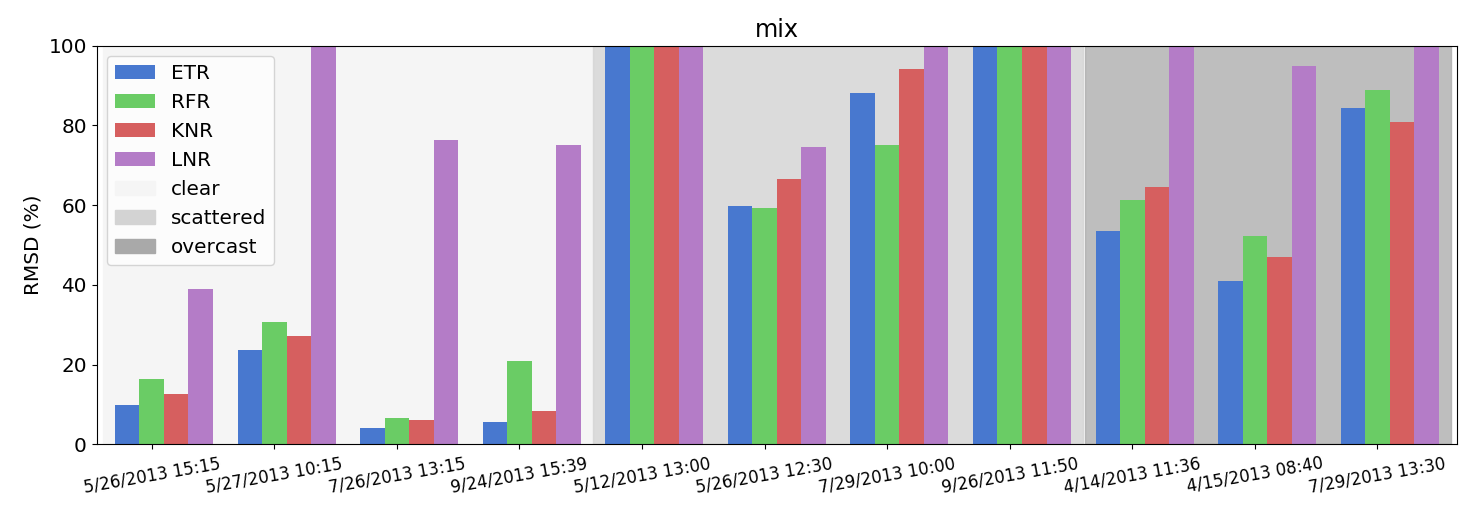
\includegraphics[width=1.0\textwidth]{img/results_mix.png}
\end{center}
\caption[error_mix] { \label{fig:error_mix}RMSD of the models trained with mix dataset, which includes all usable testing samples across all skies.}
\end{figure}

\subsection{Sky Cover}

Final results show that sky cover was extremely relevant, as initially suspected. Three of the four final models were very successful in predicting clear sky captures, shown in Tbls. \ref{tab:resultsETRclear} and \ref{tab:selectcurveerrors}, and Figs. \ref{fig:errorcurves}, \ref{fig:selectcurveratios}, and \ref{fig:wholesky}. LNR even predicted well on two clear sky captures, as mentioned in Sec. \ref{result_models}.

For scattered sky models, RFR's predictions are a surprising success (discussed below). All other models had a hard time with the data. In general, we posit that scattered skies are not predicted well by our methods (as of yet), despite the very large training set of scattered samples. There are a number of reasons why this could be. First, although lens distortions from curvature, vignetting, and even wavelength-specific variation were known to us from Saito et al.,\cite{saito_estimation_2016} we hadn't yet compensated for it in this work. Even a slight shift in sampling coordinates could severely alter the RGB values extracted from the sky images. With clear sky data, that may not be very noticeable, as the color of the sky is fairly uniform, but scattered sky clouds can vary considerably. Future work should definitely compensate for it. Second, the pixel region and weighting algorithms we used may not have been optimal for cloudy skies. Again, clear skies exhibit relatively uniform color whereas clouds and cloud/sky borders can vary, which would distort a final pixel value if weighted over a large enough kernel.

Only three overcast skies were held out for validation, and as mentioned in Sec. \ref{sec:skycover}, only 8\% of the mix dataset were overcast skies (1940 samples). So the results of this experiment on overcast skies are of low confidence. Despite that, ETR, KNR and RFR models were still able to predict one of those three captures with ~40\% RMSD. Given more data, our methods may prove successful on overcast skies as well.

Of particular interest is RFR's performance trained with a mix dataset versus a sky cover specific dataset. RFR performed worse than ETR and KNR on most validation captures when trained with mix. However, it performed equivalent or better than KNR and ETR when trained with sky cover specific data. In fact, as Fig. \ref{fig:error_skies} shows, RFR even predicted scattered skies with semi-acceptable error, something none of the other models were able to accomplish.

\begin{figure} [hbtp]
\begin{center}
\begin{tabular}{c}
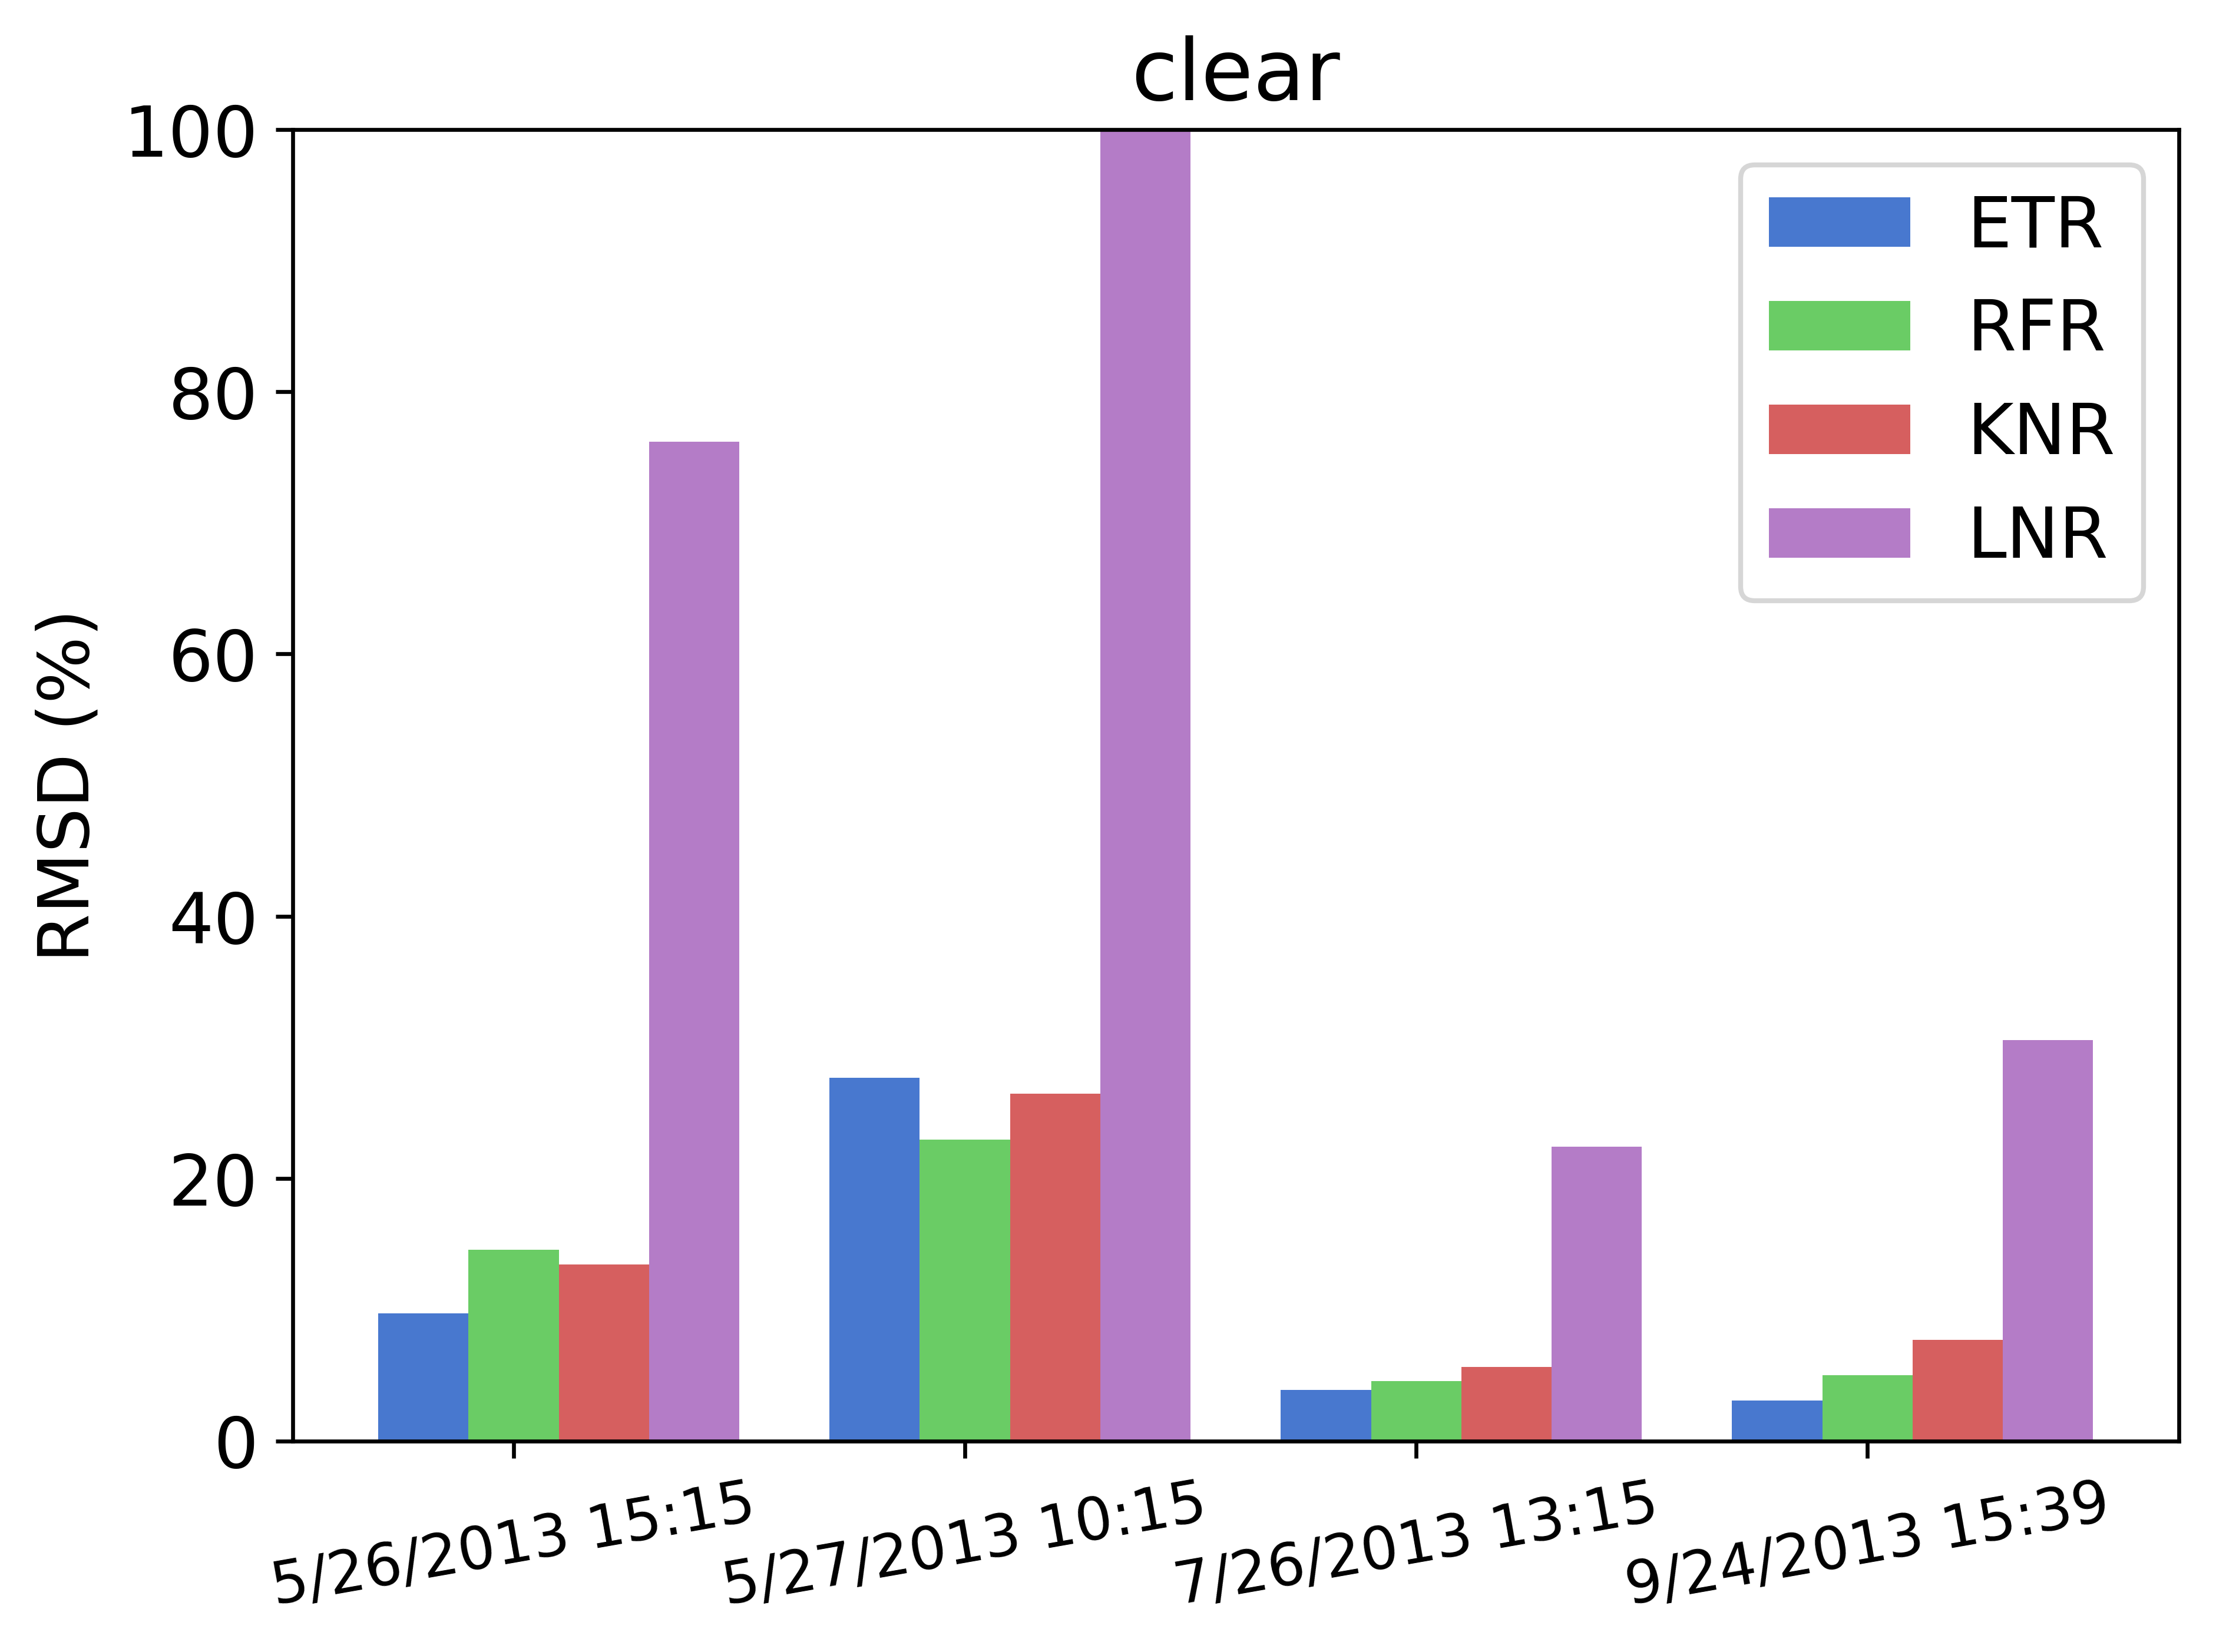
\includegraphics[width=0.32\textwidth]{img/results_clear.png}
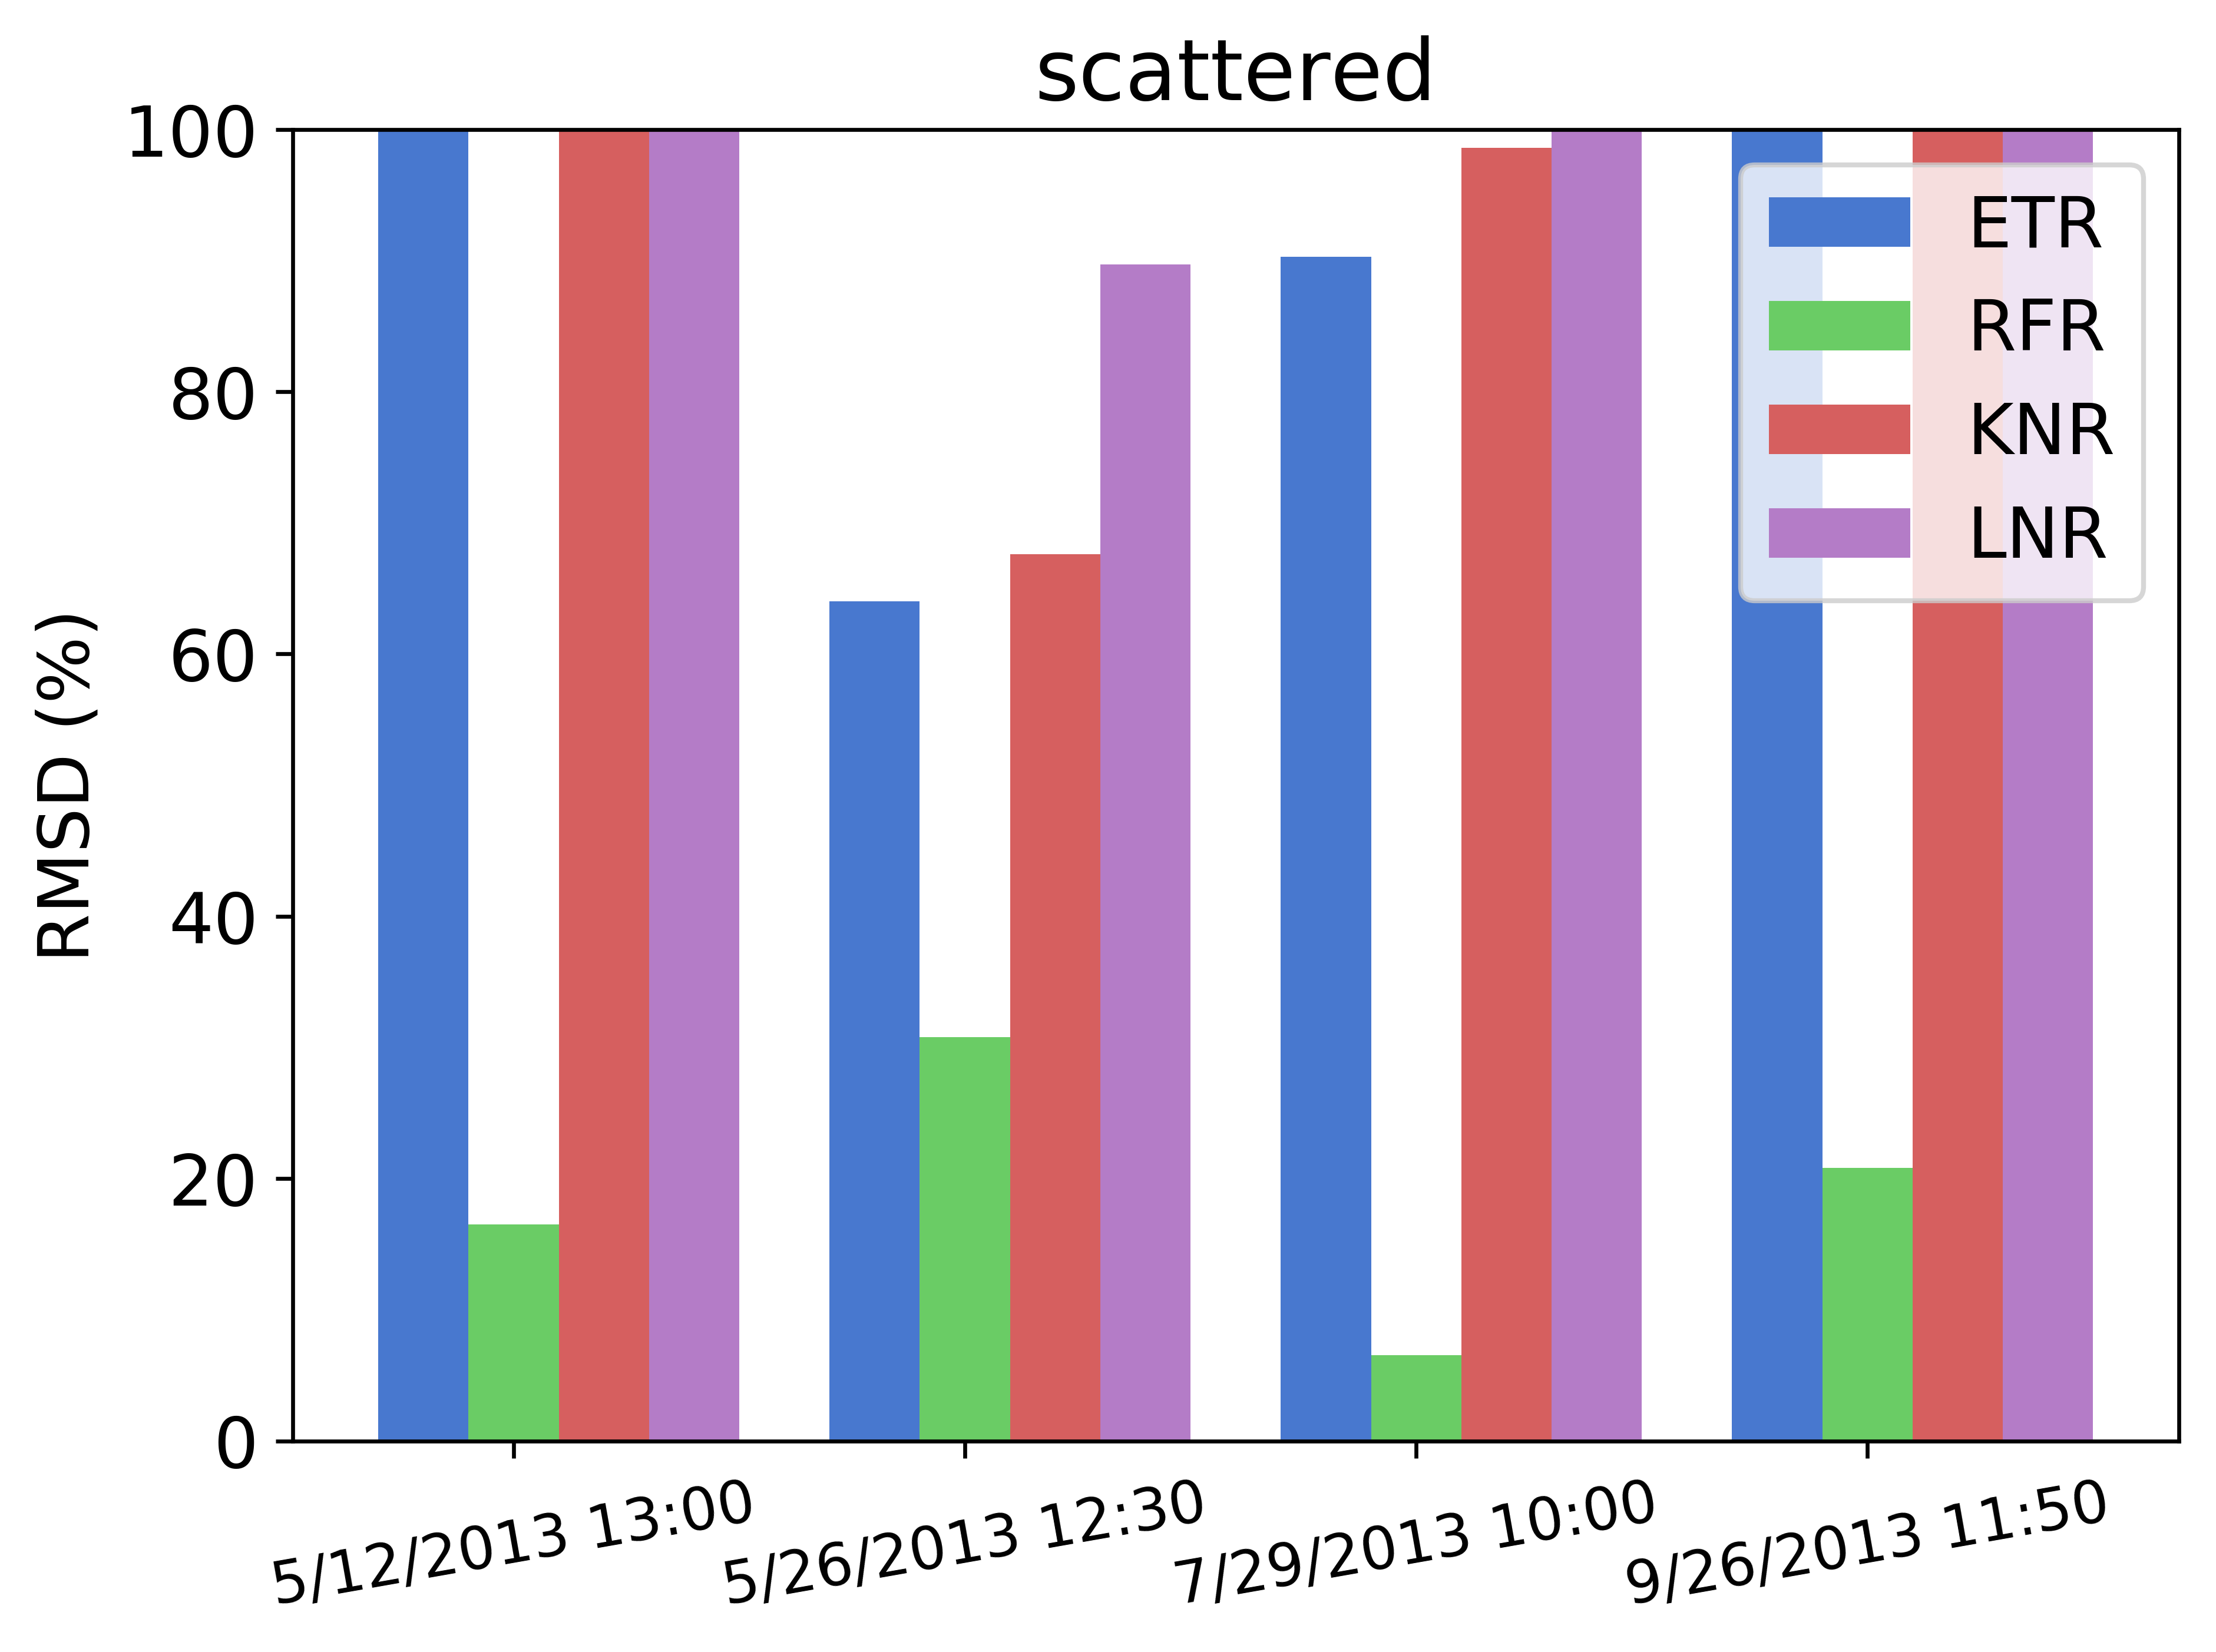
\includegraphics[width=0.32\textwidth]{img/results_scattered.png}
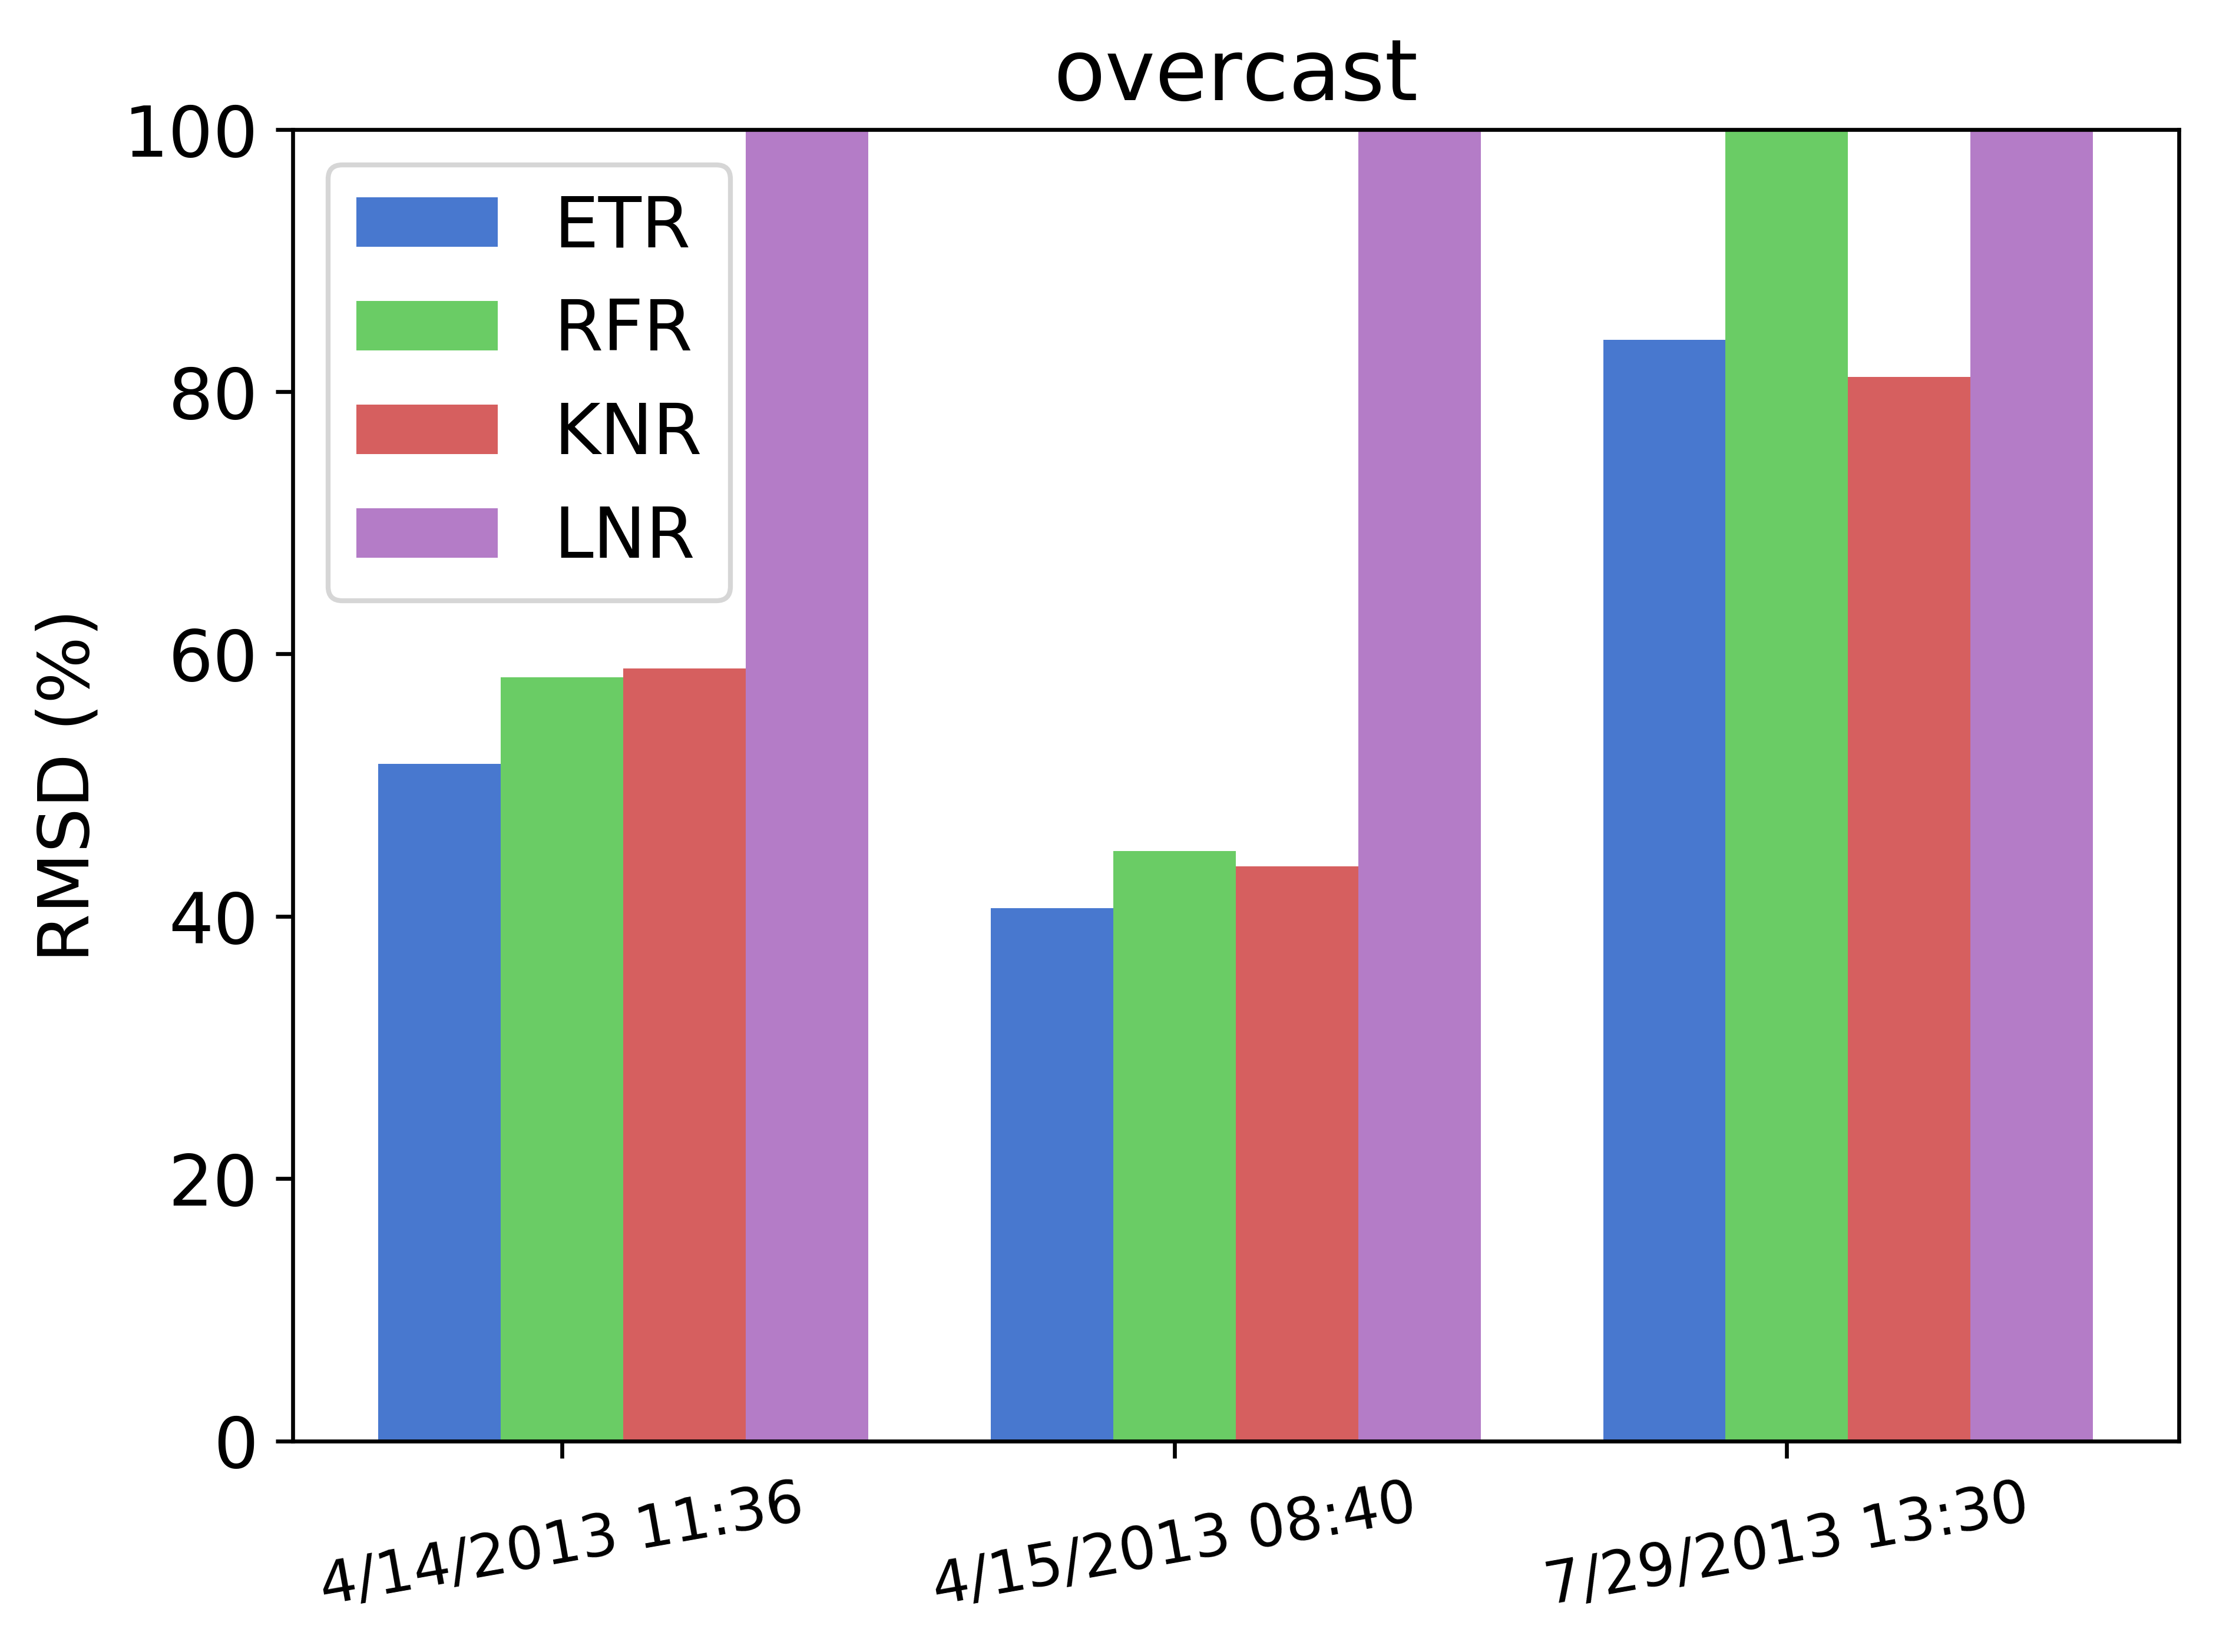
\includegraphics[width=0.32\textwidth]{img/results_overcast.png}
\end{tabular}
\end{center}
\caption[error_skies] { \label{fig:error_skies}RMSD of the models trained with sky cover specific datasets.}
\end{figure}

\begin{table}[hbtp]
\caption{Error metrics for final validation clear sky captures predicted with ETR model clear dataset.}
\label{tab:resultsETRclear}
\centering      
\begin{tabular}{cl*{4}{c}}
    \\
    \toprule
    Model & Capture & Sky & $\mathrm{R}^2$ & RMSD\\
    \midrule
    \rule[-1ex]{0pt}{3.5ex}  ETR & 05/26/2013 15:15 & CLR & 98.31\% & 9.73\% \\
    \rule[-1ex]{0pt}{3.5ex}  ETR & 05/27/2013 10:15 & CLR & 84.31\% & 27.7\% \\
    \rule[-1ex]{0pt}{3.5ex}  ETR & 07/26/2013 13:15 & CLR & 99.16\% & 3.88\% \\
    \rule[-1ex]{0pt}{3.5ex}  ETR & 09/24/2013 15:39 & CLR & 99.55\% & 3.08\% \\
%     \rule[-1ex]{0pt}{3.5ex}  ETR & 05/12/2013 13:00 & SCT & 40.12\% & 279.66\% \\
%     \rule[-1ex]{0pt}{3.5ex}  ETR & 05/26/2013 12:30 & SCT & 57.35\% & 59.87\% \\
%     \rule[-1ex]{0pt}{3.5ex}  ETR & 07/29/2013 10:00 & SCT & 0.25\% & 88.12\% \\
%     \rule[-1ex]{0pt}{3.5ex}  ETR & 09/26/2013 11:50 & SCT & 51.26\% & 104.42\% \\
%     \rule[-1ex]{0pt}{3.5ex}  ETR & 04/14/2013 11:36 & OVC & 81.07\% & 53.42\% \\
%     \rule[-1ex]{0pt}{3.5ex}  ETR & 04/15/2013 08:40 & OVC & 90.85\% & 41.10\% \\
%     \rule[-1ex]{0pt}{3.5ex}  ETR & 07/29/2013 13:30 & OVC & 46.63\% & 84.29\% \\
    \bottomrule
\end{tabular}
\end{table}

\begin{figure} [hbtp]
\begin{center}
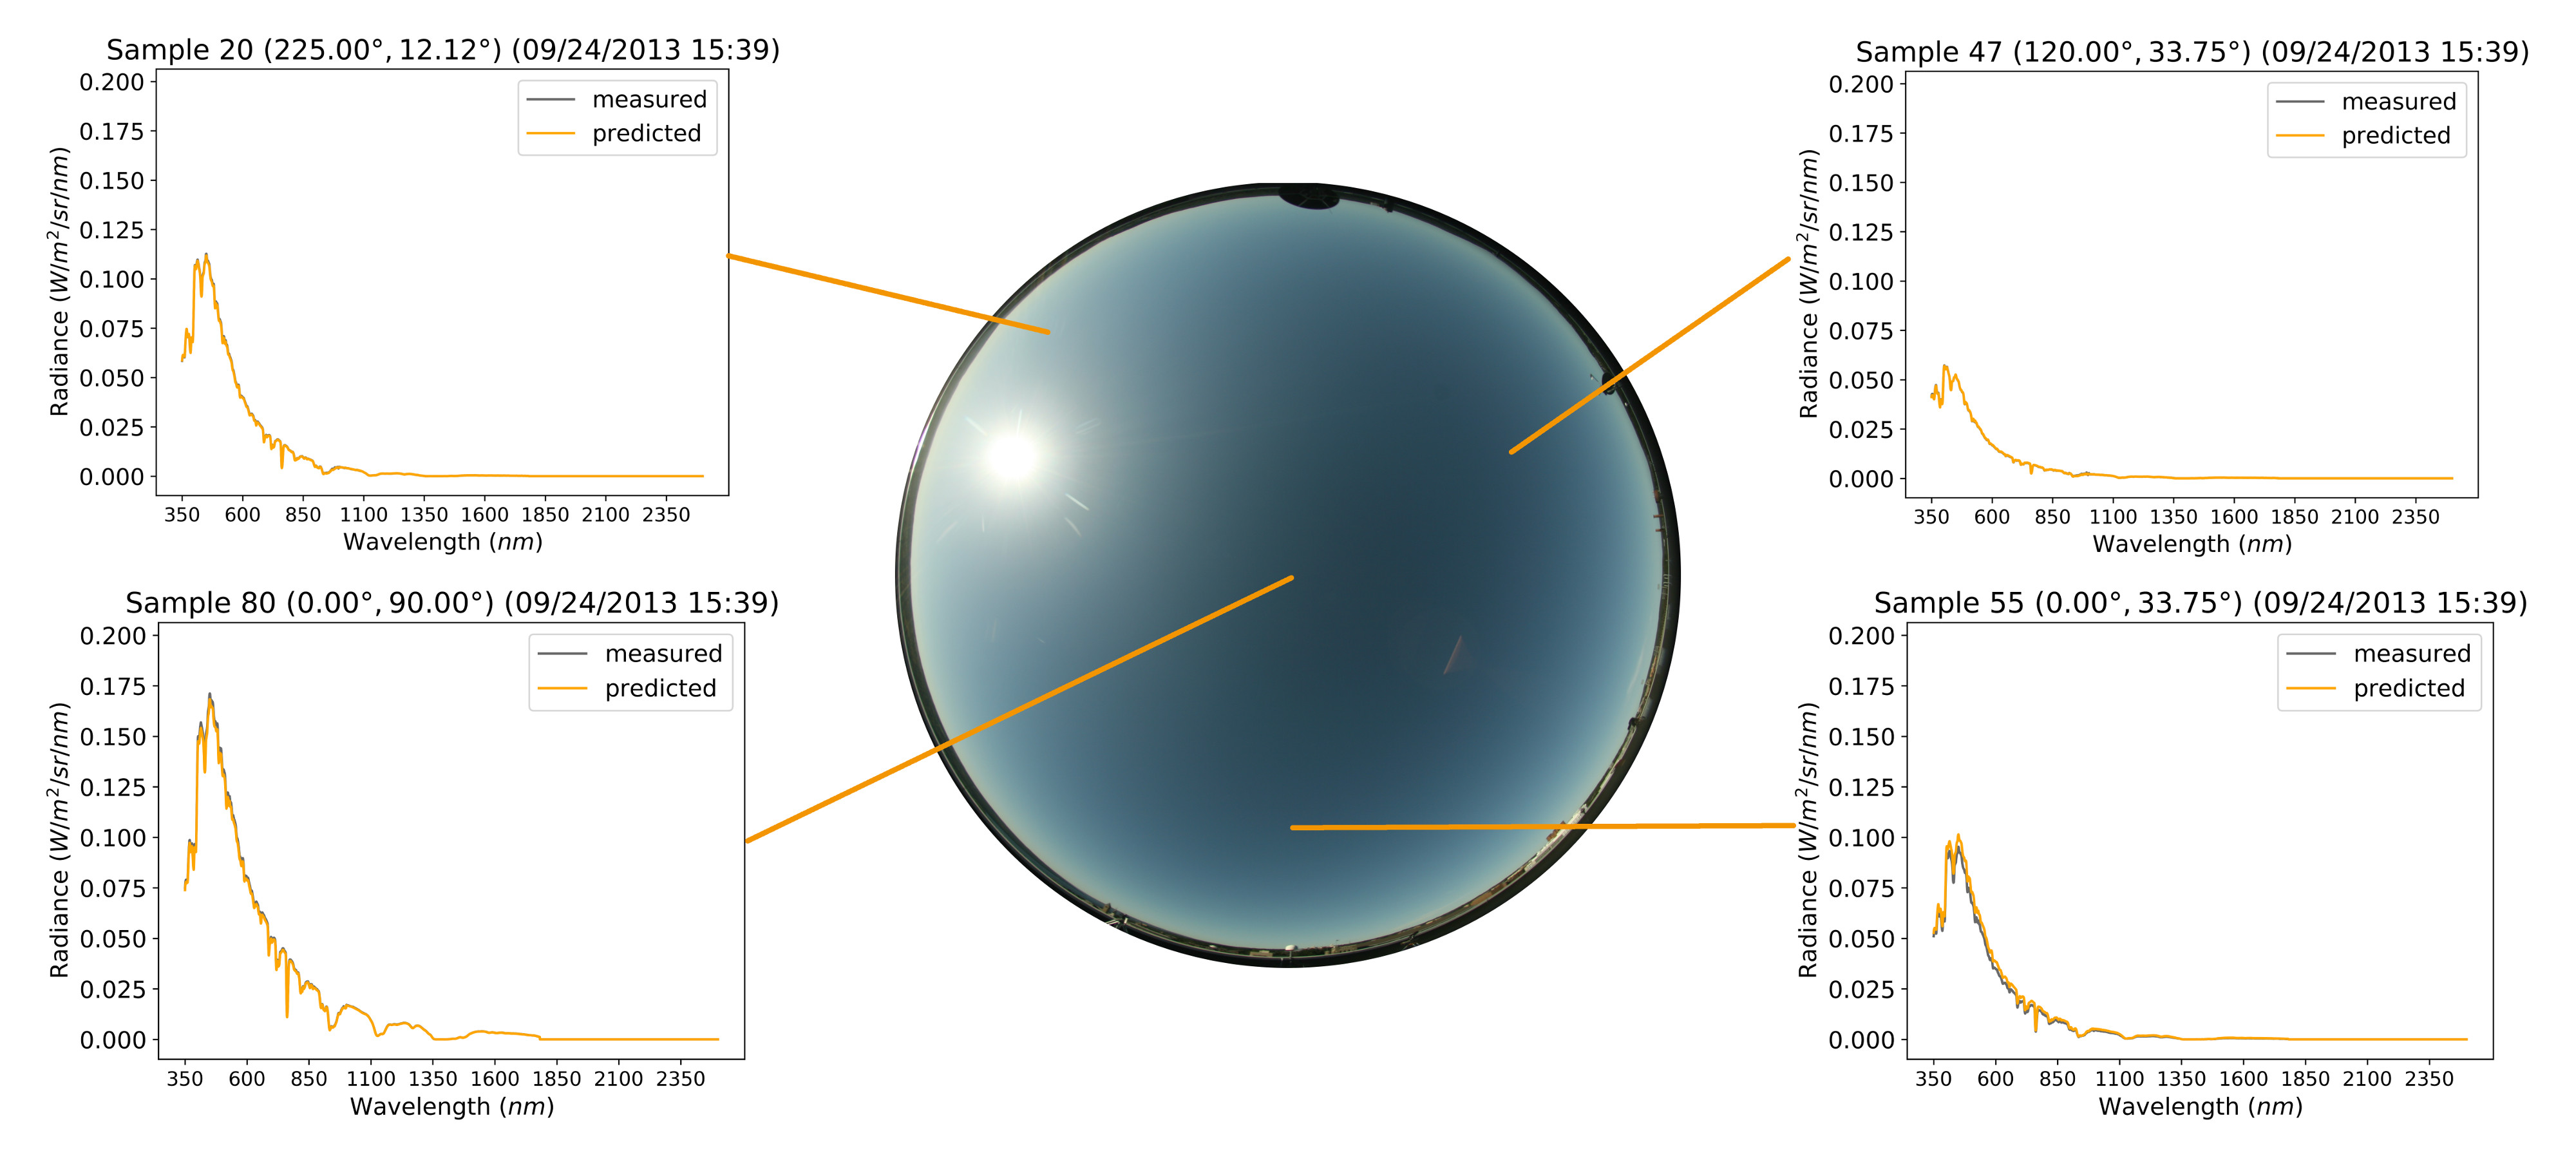
\includegraphics[width=1.0\textwidth]{img/09242013_samples.jpg}
\end{center}
\caption[errorcurves] { \label{fig:errorcurves}Select samples from clear sky capture 09/24/2013 15:39 predicted with ETR model clear dataset. \\ Video 1.~~http://dx.doi.org/doi.number.goes.here}
\end{figure}

\begin{figure} [hbtp]
\begin{center}
\begin{tabular}{c}
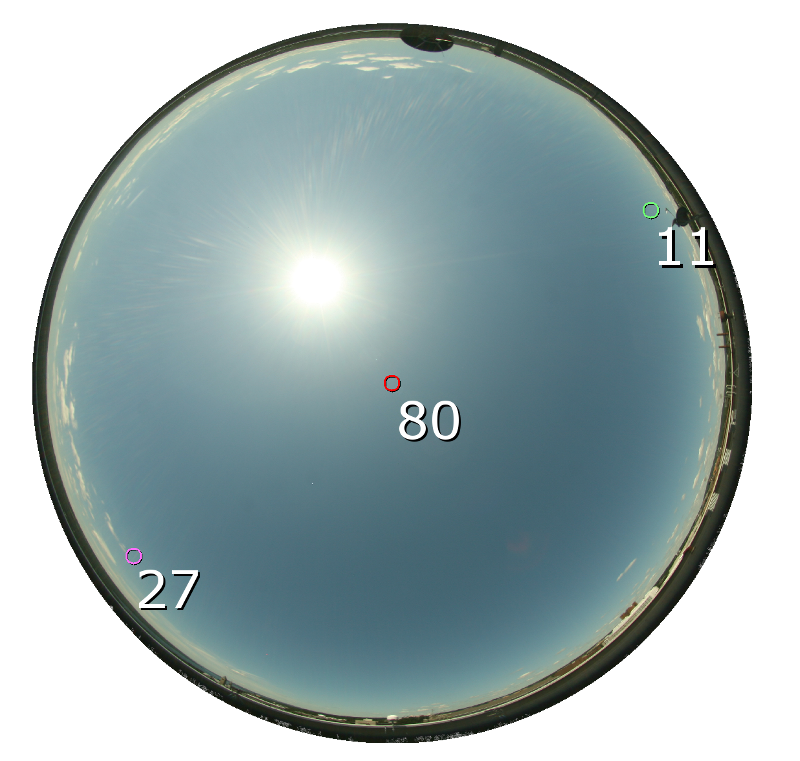
\includegraphics[width=0.44\textwidth]{img/results_072613_sky.png}
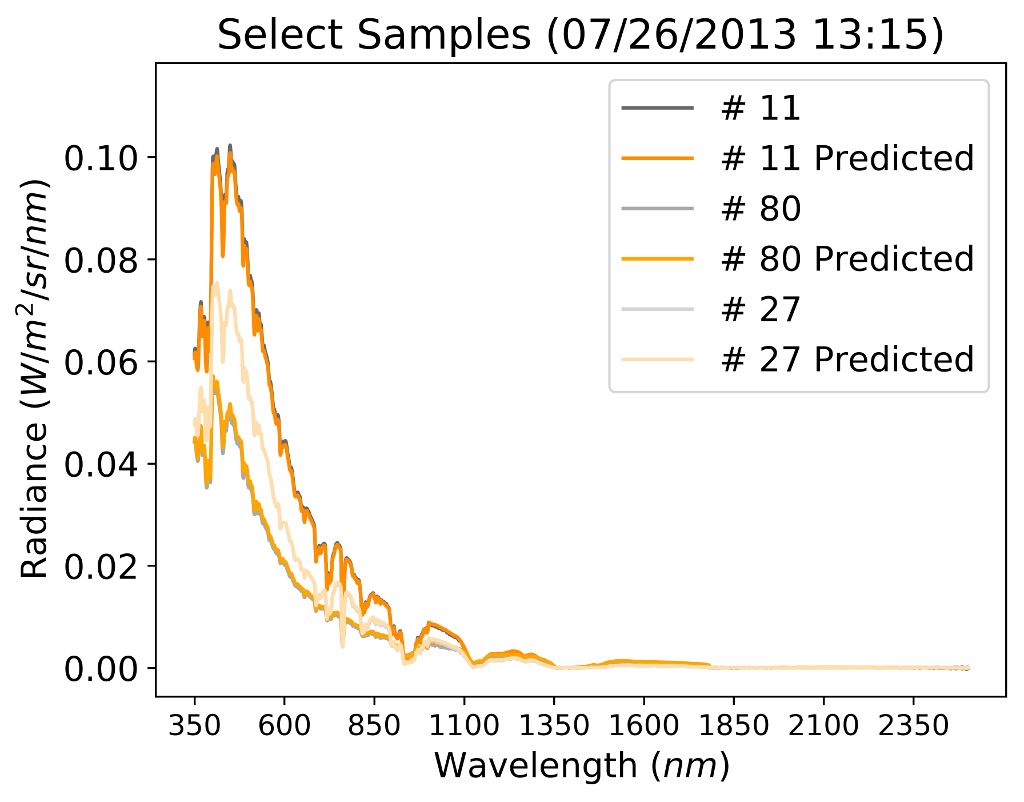
\includegraphics[width=0.54\textwidth]{img/results_072613_samples.png}
\end{tabular}
% \begin{tabular}{c}
% \includegraphics[width=0.24\textwidth]{img/results_predicted.jpg}
% \includegraphics[width=0.24\textwidth]{img/results_predicted.jpg}
% \includegraphics[width=0.24\textwidth]{img/results_predicted.jpg}
% \includegraphics[width=0.24\textwidth]{img/results_predicted.jpg}
% \end{tabular}
\end{center}
\caption[selectcurveratios] { \label{fig:selectcurveratios}Actual vs predicted radiance distributions for 3 select samples captured on 07/26/2013 13:15. Sample (80) is at the zenith, while (11) and (27) are near the horizon.}
\end{figure}

\begin{table}[hbtp]
\caption{Error metrics of actual vs predicted radiance curves for three select samples shown in Fig. \ref{fig:selectcurveratios} .}
\label{tab:selectcurveerrors}
\centering
\begin{tabular}{*{6}{c}}
    \\
    \toprule
    Sample Index & Coordinates & $\mathrm{R}^2$ & RMSD \\
    \midrule
    11 & $(123.75\degree,~12.1151\degree)$ & 99.97\% & 1.95\% \\
    27 & $(315.0\degree,~12.1151\degree)$ & 100.00\% & 0.57\% \\
    80 & $(303.75\degree,~90\degree)$ & 99.89\% & 1.92\% \\
    \bottomrule
\end{tabular}
\end{table}

\subsection{Whole Sky}

This work attempted to learn and predict collections of whole sky angular dependent radiance distribution curves for real-time application, because of the high demand across multiple disciplines for spectral illumination. Figs. \ref{fig:errorcurves}, \ref{fig:selectcurveratios}, and \ref{fig:wholesky} show that this is certainly possible with clear skies. All four holdout validation captures were predicted with success, three under 10\% error.

\begin{figure} [hbtp]
\begin{center}
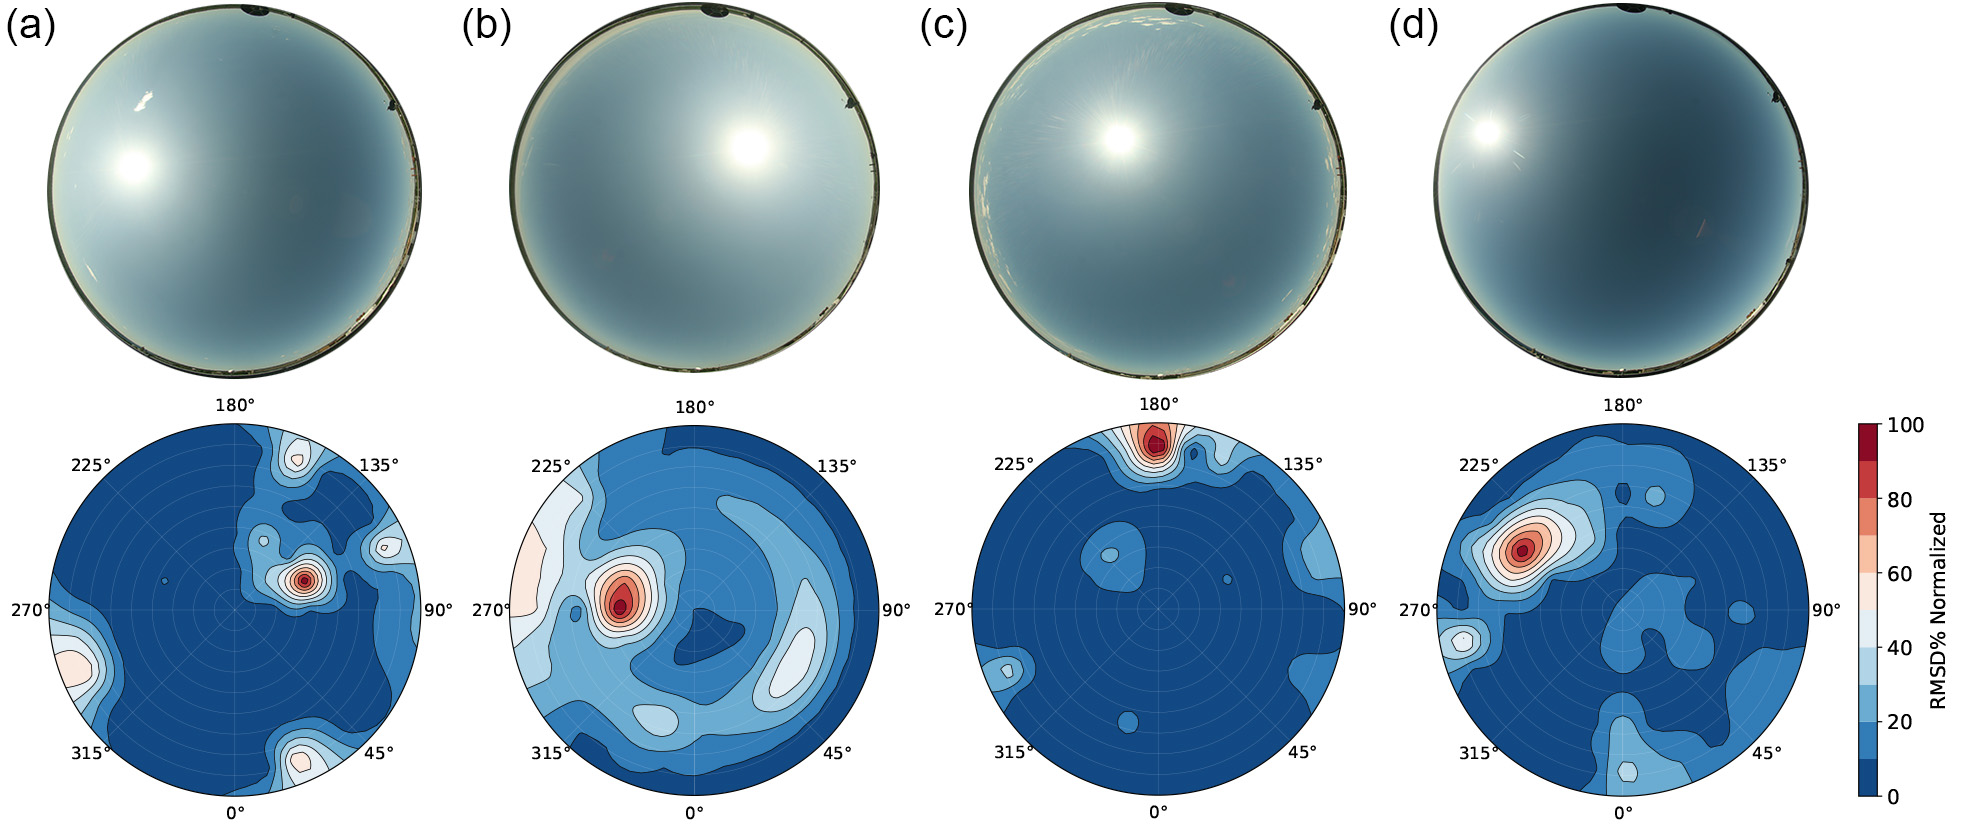
\includegraphics[width=1.0\textwidth]{img/results_wholeskyerrors.jpg}
\end{center}
\caption[wholesky] { \label{fig:wholesky}Demonstration of whole sky accuracy from holdout test data using ETR model trained on clear dataset. These captures correlate with overall error reported in Fig. \ref{fig:error_skies} and Tbl. \ref{tab:resultsETRclear}. This figure shows normalized RMSD\% for captures (a) 05/26/2013 15:15, (b) 05/27/2013 10:15, (c) 07/26/2013 13:15, and (d) 09/24/2013 15:39. We compare the generated spectral data with the captured data. (No samples from these captures were used for training.)}
\end{figure}
